

\subsection{Developer Validation}
\label{subsec.opencard}

To further validate the influential software changes dataset that we have
collected with our intuition-based post-mortem metrics, we perform a large-scale developer study. Instead of asking developers to confirm each identified
commit, we must summarize the commits into categories. To that end, we
resorted to open-card sorting~\cite{Nielsen95}, a well known, reliable and
user-centered method for building a taxonomy of a system~\cite{boxesandarrows}.
Card sorting helps explore patterns on how users would expect to find content
or functionality. In our case, we use this technique to label influential
software changes within categories that are easily differentiable for
developers.

We consider open-card sorting where participants are given cards showing
description of identified influential software changes\footnote{We consider
all 177 influential software changes from the post-mortem analysis.} without
any pre-established groupings. They are then asked to sort cards into groups
that they feel are acceptable and then describe each group. We performed this
experiment in several iterations: 
\begin{itemize}
	\item first, two authors of this paper provided individually their group descriptions, based on the 177 influential changes identified from the post-mortem analysis.
	\item  second, the two authors then met to perform another open-card sorting with cards containing their agreed group descriptions. Table~\ref{tab:cards} enumerates the 28 cards that were then summarized.
	\item Finally, a third author, with more experience in open-card sorting, joined for a final group open-card sorting process which yielded 12 categories of influential software changes.
\end{itemize}
 

The influential software changes described in the 12 categories span over
four software maintenance categories initially defined by Lientz {\em et
al.}~\cite{Lientz:1978:CAS:359511.359522} and updated in ISO/IEC 14764. Most
influential software changes belong to the {\em corrective changes} category.
Others are either {\em preventive changes}, {\em
adaptive changes} or {\em perfective changes}. Finally, changes in one of our influential change categories
 can fall into more than one maintenance categories. We refer to
them as {\em cross area changes}.



\textbf{Developer assessment.}
We then conduct a developer survey to assess the relevance of the 12 categories of influential changes that we describe. 
The survey participants have been selected from data collected in the GHTorrent project~\cite{Gousi13} which contains history
archives on user activities and repository changes in GitHub. We consider active developers (i.e., those who have contributed in the latest changes recorded in GHTorrent) and focus on those who have submitted comments on other's commit. We consider this to be an indication of experience with code review. The study\footnote{Survey form at \url{https://goo.gl/V2g8OE}} was sent to over 1952 developer email addresses. After one week waiting period, only 800 email owners opened the mail and 144 of them visited the survey link. Finally 89 developers volunteered to participate in the survey. 66 (i.e., 74\%) of these developers hold a position in a software company or work in freelance. Nine respondents (10\%) are undergraduate students and eight (9\%) are researchers. The remaining six developers did not indicate their current situation. In total, 78\% of the participants confirmed having been involved in code review activities. 26 (29\%) developers have between one and five years experience in software development. 29 (33\%) developers have between five and ten years of experience. The remaining 34 (38\%) have over ten years of experience. 

In the survey questionnaire, developers were provided with the name of a category of influential software changes, its description and an illustrative example from our dataset (we provided the same example for each category to every participant). The participant was then requested to assess the relevance of this category of changes as influential software using a Likert scale between {\tt 1:very influential} and {\tt 5:unimportant}. Figure~\ref{fig:survey} summarizes the survey results. For more detailed description of the categories, we refer the reader to the project web site (see Section ``Availability'').

The survey results suggest that:
\begin{itemize}
	\item According to software developers with code review experience, all 12 categories are about important changes: 7 categories have an average agreement of 2 (i.e., Influential), the remaining 5 categories have an average of 3 (i.e., potentially influential). Some (e.g.,  ``domino changes'' and ``changes fixing pervasive bugs'') are clearly found as more influential than others (e.g., ``important test case addition'').
	\item Some changes, such as ``fixes for hard to reproduce or locate bugs'', are not as influential as one might think.
	\item Developers also suggested two other categories of influential changes: {\em Documentation changes} and {\em Design-phase changes}. The latter however are challenging to capture in source code repository artefacts, while the former are not relevant to our study which focuses on source code changes.
\end{itemize}

With this study we can increase our confidence in the dataset of influential
software changes that we have collected. The examples listed in Section~\ref{sec:intro} can be categorized: `\textit{Adding a new lock mechanism}' to `new key features', `\textit{Changing build configurations}' to `fix configuration bugs', and `\textit{Improving performance for a specific environment}' to `fix pervasive bugs' or `fix non-functional bugs'.
%
We thus consider leveraging on the
code characteristics of these identified samples to identify more influential
changes.


%\begin{sidewaysfigure}[ht]
\begin{landscape}

 
 \begin{table}
 \centering
 \scriptsize
 	\begin{tabular}{l|r}
 	\bf Card description & \bf Example commit description (only when not summary needs explanation) \\
 	\hline
 	\hline
 		Implementation of a long-awaited feature & \\ \hline
 		Change which was discussed at length as solving a bug that was very hard to reproduce &	\\ \hline
 		trivial fixes that has high impact on basic requirements for system functionality & (e.g., in commons-compress, simple fixes but it can prevent filepath encoding problems)	\\ \hline
 		Bug fix of a key feature in library & \\ \hline
 		\multirow{2}{*}{Bug fix of a bug that manifests itself only in corner-cases} & (e.g., This fix prevents data integrity violations, which cannot be revealed unless accessing missing data.)\\
 		& Bug fix to prevent an infinite loop when API reading input stream encounters an unmappable character \\
 		\hline
 		Replacement of key functionality code to improve usability & \\ \hline
 		Fix for a regression error that is hard to reproduce and that & (e.g., the change is about exception handling (whether it should be 	caught in the program and which place). \\ 
 		occurs in specific, but popular, environment  &This is not easy to reproduce. It happens in Google App Engine and the previous version works correctly.) \\ \hline
 		Fix for an API bug - the API is used pervasively	 & \\\hline
		New feature that was discussed at length	 & \\\hline
 		New feature that implements as an API a functionality that developers 		&	\\
 		implement regularly in an ad-hoc manner in their own code & \\ \hline
		Non-functional bug fix for speciific popular API -- leads to debate & (e.g., This change fixes a performance bug which affects Android applications. This change leads \\
&  to a long 	debate	since people have different opinions on this issue. The repaired method is popular.)\\ \hline
Change reverting a bug fix to a key functionality & \\ \hline
Controversial change that is debated and then reverted &\\\hline
Fix for a bug that affects many clients/components/applications (i.e., core component) &\\\hline
Fix to a Blocking Bug & \\\hline
Fix for non-functional defect & (e.g., Performance defect --- adding multicores could not improve the performance.)	\\
New API implementation for future applications & \\\hline
Fix of dependency problems for compilation & \\\hline
Fix of configuration errors & (e.g., New build references in POM files and assembly references)	\\\hline 
Fix of a trivial bug, but which appears in several different components 		& https://github.com/wildfly/wildfly/commit/eea5d5fe34e9e7c67f076cae81fec6ebf06626af	 \\ \hline
-- leads to debate and verification of all source code & \\ 
\multirow{2}{*}{Fix a bug that is not easy to locate} & (e.g., Yes, this change releases the hang (not failing nor crashing)	\\ 
&  of a test case. A test case hang can block maven building. \\ \hline
Change that overhauls an important module/file & \\ \hline
Change that add test cases to avoid specific important functional bugs & \\ \hline
Changefor improvement of implementation by creation of new exception class& \\ \hline
Change in nightly process management& \\ \hline
Bug fix that finalizes/corrects previous fix in API& \\ \hline
Changes that lead to several collateral changes (including reverting, new API mapping)& \\ \hline
 	\end{tabular}
 	\caption{Cards after the second-round of open-card sorting}
 	\label{tab:cards}
 \end{table}
 
 
 \begin{figure}
 \centering
\scriptsize
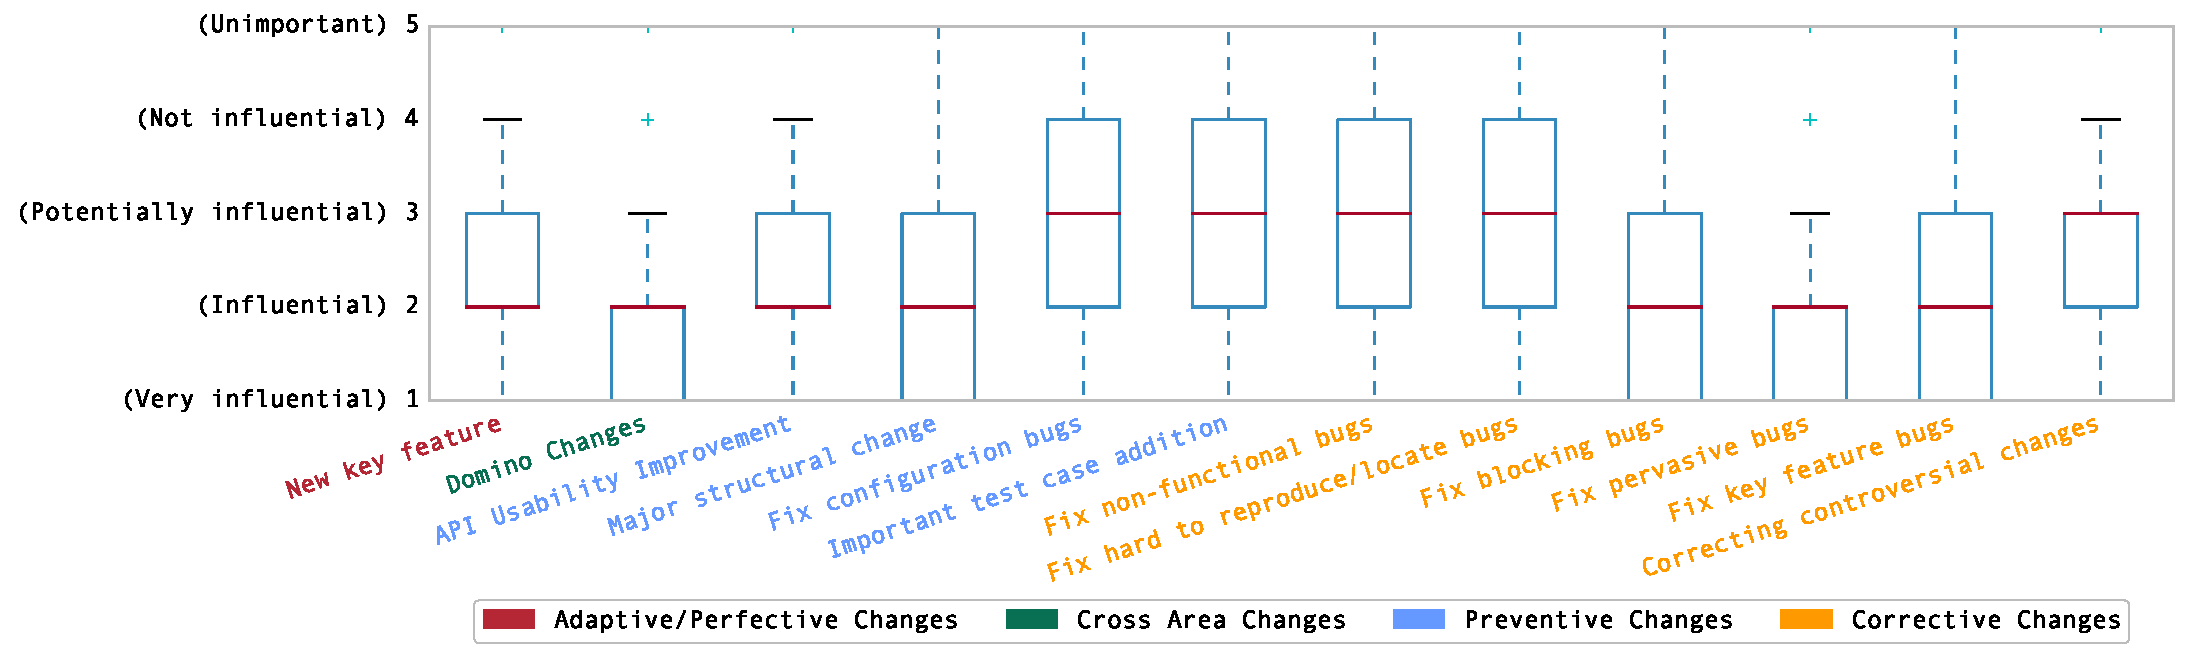
\includegraphics[width=\linewidth]{fig/response-boxplot.pdf}
\caption{Survey results on different categories of Influential Changes.}
\label{fig:survey}
%\end{sidewaysfigure}
 \end{figure}

\end{landscape}

